\chapter{Methods \label{Chapter-Methods}}

\section{Dataset}

The data we used in this work came from the Multi-Ethnic Study of Atherosclerosis (MESA) \cite{chen2015racial}, a large-scale sleep study aimed to investigate correlations between sleep quality, cardiovascular health, SDB, and other factors across different ethnic groups.
Over 6,800 men and women from six different US communities were approached in the initial examination. For the final sleep exam ten years later, 288 participants were ineligible\footnote{due to undergoing apnea treatment, living to far away, or other reasons}, roughly 2,700 were not contacted, and roughly 1,500 refused to participate. From the 2,261 participants undergoing the sleep exam, 2,060 had full-night PSG recordings, 2,156 had actigraphy data, and 2,240 completed a sleep questionnaire.

To obtain ground-truth SDB events, we used the automatic Somnolyzer scoring system \cite{anderer2022automated}, which scored the respiratory events based on the recommended criteria from the American Academy of Sleep Medicine (AASM) \cite{troester2023aasm}: apnea events were defined as a 90\% or greater reduction in airflow for at least 10 seconds, while hypopnea events were defined as a 30\% or greater reduction in airflow for at least 10 seconds, with either a $\geq 3\%$ oxygen desaturation or an associated arousal.

To leverage the different expressions of respiratory events in different sleep stages, we explored the use of sleep stage classes as an additional input to our model. To do so, we used a previously developed sleep staging algorithm created by Bakker et al. \cite{bakker2021estimating}, restricted to only use PPG signals as inputs, ensuring that our algorithm doesn't depend on signals outside of the finger-worn PPG sensor setup.
We achieved a pooled Cohen's Kappa of 0.55 when measuring agreement between the PPG-predicted hypnogram\footnote{Bakker's model combined N1 and N2 stages into one, resulting in four stages: Wake, N1/N2, N3, and REM. For calculating the Kappa, Somnolyzer scorings were adjusted to the same format} and the the ground-truth Somnolyzer PSG-derived hypnogram, showing moderate agreement. A detailed performance comparison can be found in Appendix \ref{Apx-Pred-Hypnogram}.

Filtering the MESA participants for those with PPG and SpO2 data, Somnolyzer scorings, and available predicted hypnograms, we ended up with a dataset size of 1,880 participants. Table \ref{tab:dataset-demographics} shows the demographic distribution and sleep times of our dataset subset together with the folds, generated for cross validation as discussed later in this chapter.
To assess SDB severity, the AHI is often categorized into four classes. These so called severity classes are defined as follows: Normal (AHI $<$ 5), Mild (5 $\le$ AHI $<$ 15), Moderate (15 $\le$ AHI $<$ 30), and Severe (AHI $\ge$ 30).
Table \ref{tab:dataset-ahi} shows their distribution.
The number of different apnea classes is shown in Table \ref{tab:dataset-apnea-classes}.

\renewcommand{\arraystretch}{1.5}
\begin{table}
    \centering
    \begin{tabular}{p{1cm} p{1cm} p{1.7cm} p{1.7cm} p{1.7cm} p{1.7cm}}
        Fold & N & Age \newline (years) & BMI \newline ($kg/m^2$) & Sex \newline (N male) & TST \newline (h) \\
        \hline
        1 & 470 & $70\pm9$ \newline \textbf{[55, 90]} & $29\pm5$ \newline \textbf{[19, 48]} & 228 \newline (48.5\%) & $6.2\pm1.36$ \newline \textbf{[1.7, 10]} \\
        2 & 470 & $70\pm9$ \newline \textbf{[54, 90]} & $29\pm6$ \newline \textbf{[17, 56]} & 208 \newline (44.3\%) & $6.2\pm1.36$ \newline \textbf{[1.6, 10]} \\
        3 & 470 & $69\pm9$ \newline \textbf{[55, 90]} & $29\pm5$ \newline \textbf{[16, 50]} & 229 \newline (48.7\%) & $6.2\pm1.47$ \newline \textbf{[0.7, 10]} \\
        4 & 470 & $69\pm9$ \newline \textbf{[55, 90]} & $28\pm5$ \newline \textbf{[17, 50]} & 210 \newline (44.7\%) & $6.2\pm1.32$ \newline \textbf{[0.9, 10]} \\
        \hline
        Full & 1880 & $69\pm9$ \newline \textbf{[54, 90]} & $29\pm6$ \newline \textbf{[16, 56]} & 875 \newline (46.5\%) & $6.2\pm1.38$ \newline \textbf{[0.7, 10]} \\
    \end{tabular}
    \caption{Demographic distribution and sleep times of the MESA dataset subset. Format for Age, BMI, and TST is mean $\pm$ std [min, max]. \label{tab:dataset-demographics}}
\end{table}

\renewcommand{\arraystretch}{1.5}
\begin{table}
    \centering
    \begin{tabular}{p{1cm} p{2cm} p{1.5cm} p{1.5cm} p{1.5cm} p{1.5cm}}
         &  & \multicolumn{4}{c}{Severity Class} \\
        \cline{3-6}
        Fold & AHI & normal & mild & moderate & severe \\
        \hline
        1 & $22.2\pm18.3$ \newline \textbf{[0.4, 100]} & 61 & 153 & 136 & 120 \\
        2 & $22.0\pm18.3$ \newline \textbf{[0.3, 93]} & 61 & 151 & 134 & 124 \\
        3 & $21.3\pm17.1$ \newline \textbf{[0.4, 95]} & 61 & 151 & 138 & 120 \\
        4 & $22.0\pm18.3$ \newline \textbf{[0.4, 107]} & 61 & 150 & 140 & 119 \\
        \hline
        Full & $21.9\pm18.0$ \newline \textbf{[0.3, 107]} & 244 & 605 & 548 & 483 \\
    \end{tabular}
    \caption{AHI and severity class distribution accross folds and full dataset subset. Format for the AHI is mean $\pm$ std [min, max]. \label{tab:dataset-ahi}}
\end{table}

\renewcommand{\arraystretch}{1.5}
\begin{table}
    \centering
    \begin{tabular}{p{1cm} p{1.7cm} p{1.7cm} p{1.7cm} p{1.8cm}}
        Fold & obstructive \newline apnea & central \newline apnea & mixed \newline apnea & hypopnea \\
        \hline
        1 & 15k (24\%) & 4k (7\%) & 1k (2\%) & 42k (67\%) \\
        2 & 16k (26\%) & 4k (6\%) & 1k (2\%) & 42k (66\%) \\
        3 & 15k (24\%) & 3k (6\%) & 1k (2\%) & 41k (67\%) \\
        4 & 17k (26\%) & 4k (6\%) & 1k (2\%) & 42k (66\%) \\
        \hline
        Full & 63k (25\%) & 16k (6\%) & 5k (2\%) & 167k (67\%) \\
    \end{tabular}
    \caption{Total number of apnea events per fold and in total. Important to note is the imbalance of the different apnea types, especially the underrepresentation of central and mixed apnea. \label{tab:dataset-apnea-classes}}
\end{table}

\section{Signals and Preprocessing}

We used the PPG and SpO2 signals from the MESA dataset, which were recorded at 256Hz and 1Hz, respectively. A third input to the model is the hypnogram from Bakker et al. \cite{bakker2021estimating}, which was predicted at $\frac{1}{30}$Hz and on PPG only, ensuring that the model still relies solely on data it can retrieve from the PPG sensor in the real world.
We denoised the PPG signal using a lowpass filter with a cutoff frequency of 5Hz. An example of this denoising can be found in Appendix \ref{Apx-Denoise}.

To analyse the importance of correct sleep stage information, we also tested a version of the model that uses the "ground-truth" Somnolyzer hypnogram instead of the predicted one.

\subsection*{PPG Preprocessing}

To deal with the high temporal resolution of the PPG signal, we tested three different preprocessing methods that would transform the 256Hz signal into a 1Hz signal with multiple dimensions:

\begin{itemize}
    \item \textbf{Statistical}: On a 1Hz basis we extracted the mean, standard deviation, minimum, maximum, and mean peak interval of the PPG signal, resulting in a 5-dimensional representation of the PPG signal. Due to the nature of PPG showing the heartbeats at 1Hz, we used a sliding window of 5s around the 1Hz point to calculate the statistics.
    \item \textbf{Variational Autoencoder}: The Variational Autoencoder (VAE) is an unsupervised generative model that learns to encode the input data into a lower-dimensional latent space and then reconstruct it back to the original space. The VAE consists of an encoder and a decoder, where the encoder maps the input data to a distribution in the latent space, and the decoder samples from this distribution to reconstruct the input. Using the same sliding window approach as in the statistical method, we trained the VAE to reconstruct the middle 1s from the 5s input window. With that, the encoder learns to compress the input into a lower temporal dimension while preserving the relevant information. For training the main SDB detector model, this encoder is used to transform the 256Hz PPG signal into a 1Hz signal with 8 dimensions.
    \item \textbf{In-model Convolution Stack}: While the prior methods calculated the 1Hz representation of the PPG signal before training the model, we also tested a method that would use a stack of convolutions to learn the 1Hz representation during training. The convolution stack consists of five \textit{double convolution blocks} (DCB) which are composed of two 1D convolution layers with a kernel size of 3 or 5, each followed by a batch normalization layer and ReLU activation. Between these blocks are max pooling layers with a kernel size of 4 resulting in the downsampling of the signal to 1Hz, while bringing the number of channels up from 1 to 8.
\end{itemize}

Each preprocessing method brings the PPG signal down to 1Hz with multiple dimensions, which is then stacked together with the 1Hz SpO2 signal and the hypnogram that was upsampled to 1Hz. The input to the detection model is therefore a 1Hz signal with $2+d$ dimensions, with $d$ being the number of dimensions from the selected PPG preprocessing method(s). 

\section{Model Architecture}

The core of the detection model is an adapted version of the U-Net architecture, originally proposed for 2D image segmentation by Ronneberger et al. \cite{ronneberger2015u}. The U-Net architecture improves an encoder-decoder structure by adding skip connections between the corresponding encoder and decoder layers, which allows the model to learn both low-level and high-level features. The adapted model uses 1D convolutions on the temporal dimension instead of 2D convolutions on the width and height of images. The output of the U-Net has the same resolution as the input, which allows the model to classify each second as either part of an event or of normal breathing. This in turn allows us or the user to analyse the prediction on an event level, instead of just the AHI level, which can be important, as studies showed links between apnea event duration and health that go beyond the AHI severity classifications \cite{butler2019apnea}. Figure \ref{fig:model} shows the model architecture and the DCBs, that are also used for the preprocessing VAE.

\begin{figure}
    \centering
    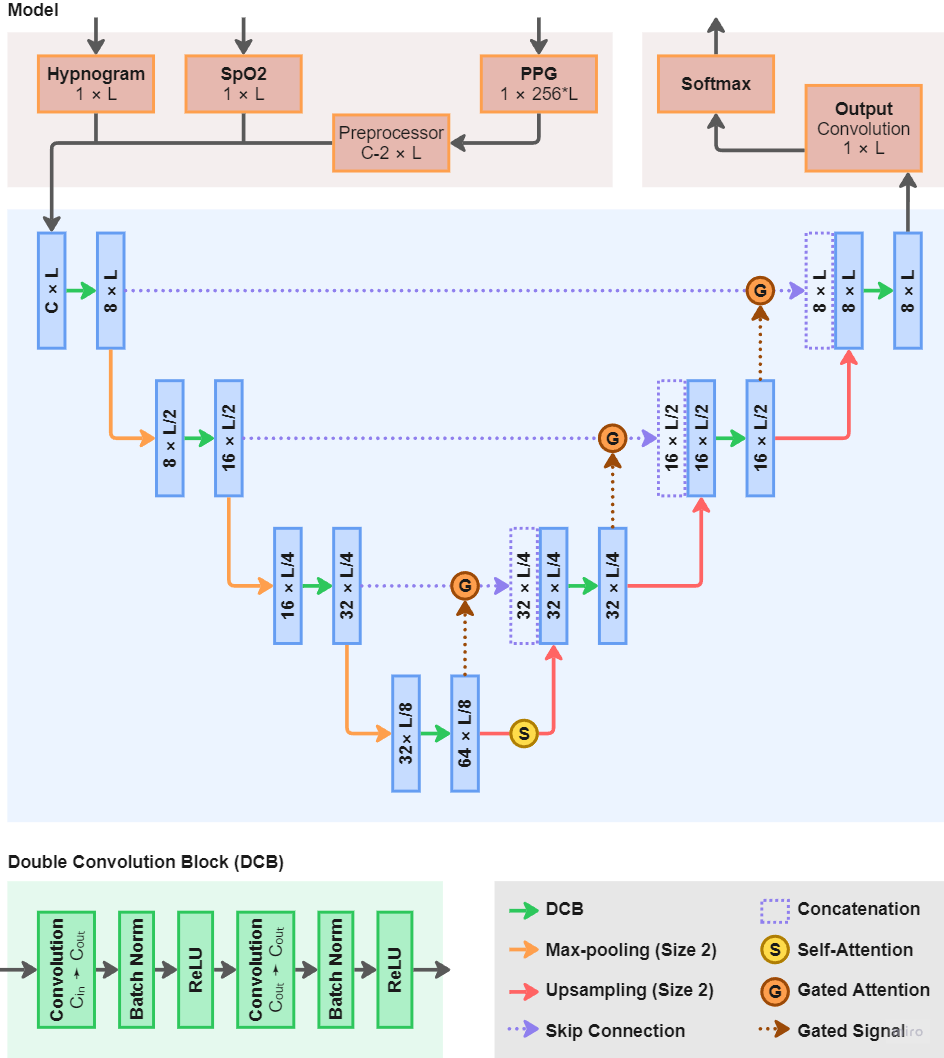
\includegraphics[width=\textwidth]{images/Model}
    \caption{Architecture of the model and shape of the data flowing through the network. $L$ is the sequence length, which is 30 minutes in our case. $C$ is the number of input features (or channels for the convolutions), with the hypnogram and SpO2 signal having one channel each, while the number of PPG channels depend on the preprocessing technique used. The convolutions kernel sizes are 3 for the DCBs and 1 for the output convolution.}
    \label{fig:model}
\end{figure}

\subsection*{Attention mechanisms}

Our model can leverage three types of attention:

\begin{itemize}
    \item \textbf{Self-Attention in the bottleneck}: The self-attention mechanism, originally proposed by Vaswani et al. \cite{vaswani2017attention}, computes relevance vectors for each input feature through their query (Q) and key (K) matrices. By multiplicating this vector with the value matrix (V), the model learns long-range dependencies throughout the sequence, making it possible to focus on the important parts of the input data. The self-attention mechanism is computed as:
    \begin{equation}
        \text{Attention}(Q, K, V) = \text{softmax}\left(\frac{QK^T}{\sqrt{d_k}}\right)V
    \end{equation}
    where $d_k$ is the dimension of the key matrix and the softmax function normalizes the attention scores, ensuring that they sum to 1.
    Using Self-Attention can increase model complexity greatly due to their quadratic complexity, which is why we apply it in the bottleneck, where the temporal resolution is at its lowest.
    \item \textbf{Attention gates}: Originally proposed for the task of medical pancreas image segmentation by Oktay et al. \cite{oktay2018attention}, attention gates are employed at the skip connections of the U-Net and help the model highlight important regions while suppressing irrelevant ones. They work by learning a gate that refines the skip connection (encoder) features before concatenation. This gate is computed from the same incoming skip connection features and the decoder features from the layer below.
    % \item \textbf{Squeeze-and-Excitation (SE) blocks}: The SE block, proposed by Hu et al. \cite{hu2018squeeze}, is a lightweight attention mechanism that computes channel-wise feature importance. It works in two parts: First, the squeeze operation creates feature maps accross the spatial dimensions using global average pooling, resulting in a 1D vector for each channel. Then, in the excitation part, two fully connected linear layers with ReLU activation transform this vector and multiply it with the input, effectively weighting the channels by importance. \todo{delete as it is not used}
\end{itemize}

\section{Training and Evaluation}

\subsection*{Cross-Validation}

To ensure statistical validity, we used a fixed seed of $42$ and a 4-fold cross-validation approach balanced for AHI severity class. In k-fold cross-validation, the dataset is split into k equal parts (called folds). One then selects one fold as the test set and trains the model on the remaining k-1 folds. This process is repeated k times, each time with a different fold as the test set, and the evaluation results on the test sets are averaged to obtain a more reliable estimate of the model's performance. This approach helps to mitigate the risk of overfitting and provides a more robust evaluation of the model's generalization ability. Figure \ref{fig:crossvalidation} illustrates the cross-validation process.
As seen in Tables \ref{tab:dataset-demographics}, \ref{tab:dataset-ahi}, and \ref{tab:dataset-apnea-classes}, the folds are not only balanced for AHI severity class, but also show a good distribution of demographic data.

\begin{figure}
    \centering
    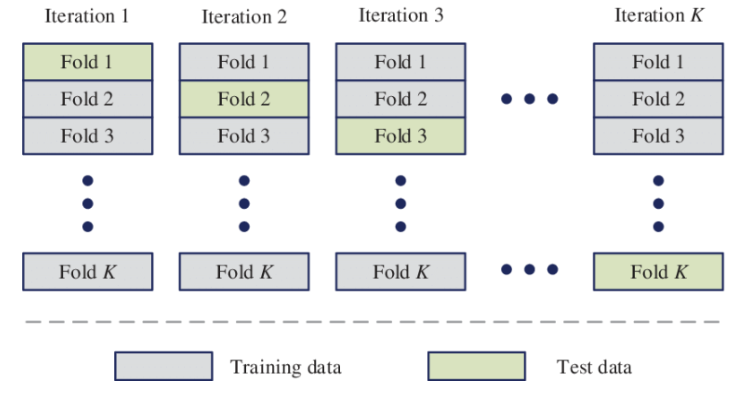
\includegraphics[width=\textwidth]{images/CrossValidation}
    \caption{Structure of a k-fold cross-validation. Source: \url{https://www.researchgate.net/figure/K-fold-cross-validation-method\_fig2\_331209203}}
    \label{fig:crossvalidation}
\end{figure}

\subsection*{Training Parameters and Setup}

The training targets are one-dimensional vectors with the same length as the input sequence, where each second is labeled as either 0, indicating normal breathing, or 1, indicating an apnea event. The final layer of the model is a sigmoid activation function, that maps each second to an event probability value between 0 and 1. During training, we optimize the binary cross-entropy loss\footnote{specifically, we use PyTorch's \texttt{nn.BCEWithLogitsLoss()}, which combines the sigmoid activation and BCE loss into one class, as it is more stable than doing these operation in sequence.} (BCE) between the predicted probabilities and the true labels. The BCE loss is defined as:
\begin{equation}
    \text{BCE} = \frac{1}{N}\sum_{i=1}^{N} [ y_i \cdot \log(p_i) + (1 - y_i) \cdot \log(1 - p_i) ]
\end{equation}
where $N$ is the number of samples (or seconds in our case), $y_i$ is the true label (0 or 1, normal or abnormal breathing), and $p_i$ is the predicted probability for sample $i$. The loss is then averaged over each batch and parsed to the optimizer, in our case the Adam optimizer with a learning rate of 0.001.

As for batching, we used randomly selected 32 30-minute segments from four different recordings each to mitigate batch overfitting on sleep patterns of a single participant.

During testing, we used a sliding window approach, were each recording was split into 30-minute segments with a 2-minute overlap \ref{fig:slidingwindow}. Model predictions were then concatenated, disregarding each first and last minute to create the final prediction for the whole night. This approach allows us to predict recordings of arbitrary length, on which metrics like the AHI can be calculated.

\begin{figure}
    \centering
    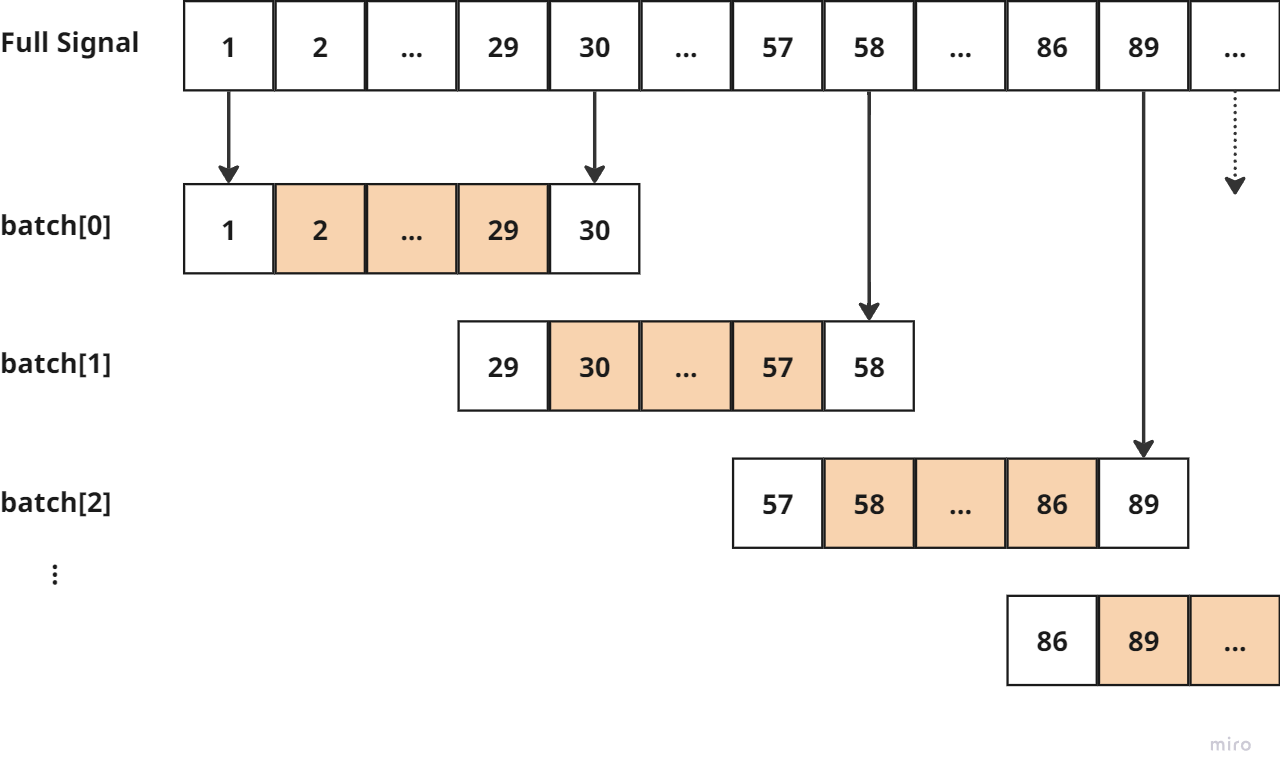
\includegraphics[width=0.75\textwidth]{images/SlidingWindow}
    \caption{Dividing the full recording into 30-minute segments with a 2-minute overlap. The first and last minute of each segment are disregarded, so that the concatenation resembles the original recording for the final prediction.}
    \label{fig:slidingwindow}
\end{figure}

Each fold has been trained on a single NVIDIA A40 GPU with 48GB VRAM with a time limit of 2 days for 30 epochs.

\subsection*{Evaluation Metrics}

Several metrics are employed to measure the performance of the model, that can be divided into three categories:

\subsubsection*{A. Event-level metrics}

To assess the model performance on an event level, regardless of the length of the night, we use the event-level metrics. They are calculated by extracting events from the predicted probabilities by thresholding the probabilities and counting each consecutive sequences of 1s as a single event. To mitigate outliers, we disregarded events shorter than 3 seconds and combined consecutive events that are less than 3 seconds apart into one event. We call this the \textit{output correction}.

Olsen et al. \cite{olsen2020robust} defined scoring rules on the event-level that are defined as follows: A predicted event, that overlaps with a true event, gets classified as a true positive (TP). If a predicted event has no overlapping true event, it gets counted as a false positive (FP). If a true event doesn't overlap with any predicted event, it gets counted as a false negative (FN). Note that there are no true negatives (TN) on the event-level. In this work, we use a more strict version of their rules, that were adjusted by Xie et al. \cite{xie2023use}, and in which each event can only be used for scoring one time. Meaning that if a predicted event overlaps with multiple true events, only one true event gets counted as TP, while the others are counted as FN. The same applies the other way around, where a true event can only be counted as TP once and other overlapping predicted events are counted as FP. A visual example can be seen Figure \ref{fig:eventscoring}. From this, we can now compute the following metrics:

\renewcommand{\arraystretch}{1.5}
\begin{table}[h!]
    \centering
    \begin{tabular}{p{1.6cm} p{2cm} p{4.4cm}}
        Metric & Calculation & Meaning \\
        \hline
        Recall \newline (Rec) & $\frac{TP}{TP+FN}$ & What \% of real events \newline got detected? \\
        Precision \newline (Pr) & $\frac{TP}{TP+FP}$ & What \% of predicted events \newline where real events? \\
        F1-score & $2 * \frac{Pr * Re}{Pr + Re}$ & Harmonic mean of \newline Precision and Recall \\
    \end{tabular}
\end{table}

\begin{figure}
    \centering
    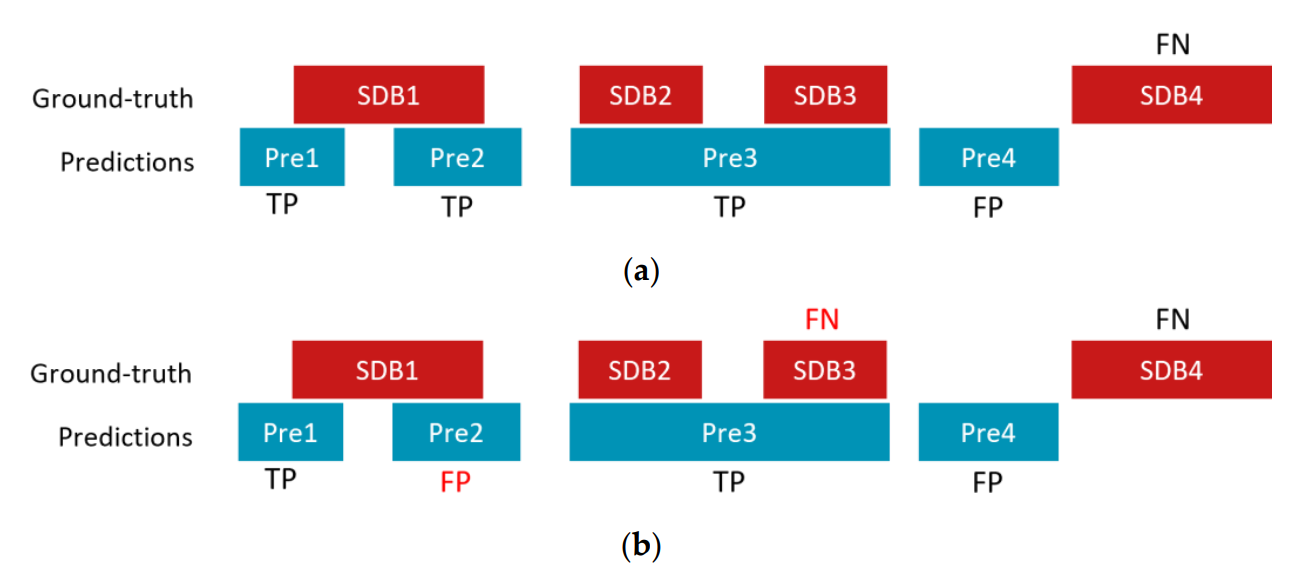
\includegraphics[width=\textwidth]{images/EventScoring}
    \caption{Example of the event scoring. (a) shows the version from Olsen et al. \cite{olsen2020robust}. (b) illustrates the extra rules of the version we use: As every pair of TPs can only be scored once, Pre2 and SDB3 are counted as FP and FN respectively. Source: Figure taken from \cite{xie2023use}.}
    \label{fig:eventscoring}
\end{figure}

As these metrics depend on the selection for a proper threshold, we \todo{we or we'll?} show these metrics as a function of the threshold.

\subsubsection*{B. AHI-level metrics}

Dividing the total number of apnea events by the TST (in hours) gives us the most common metric for SDB severity, the AHI. We compare the predicted AHI ($AHI_{pred}$) and the Somnolyzer AHI ($AHI_{true}$) using the following metrics:

\begin{itemize}
    \item Plotting $AHI_{pred}$ against $AHI_{true}$ shows their correlation which can also be expressed in the \textbf{Root Mean Square Error} (RMSE) and the \textbf{$R^2$} value. RMSE is calculated as:
    \begin{equation}
        RMSE = \sqrt{\frac{1}{n}\sum_{i=1}^{n}(AHI_{pred} - AHI_{true})^2} 
    \end{equation}
    where n is the number of samples (or participants AHIs in our case). $R^2$ is calculated as:
    \begin{equation}
        R^2 = 1 - \frac{\sum_{i=1}^{n}(y_i - f_i)^2}{\sum_{i=1}^{n}(y_i - \bar{y}_i)^2}
    \end{equation}
    where $y_i$ is the i-th predicted AHI, $\bar{y}_i$ is the mean of the predicted AHIs, and $f_i$ is the i-th true AHI. The $R^2$ value ranges from 0 to 1, where 0 indicates no correlation and 1 indicates a perfect correlation.
    \item The \textbf{Bland-Altman plot} is another way to visualize agreement by plotting the difference between the two AHI values against their mean. This allows us to see the bias, defined as the mean difference, and limits of agreement, defined as the bias $\pm$ 1.96 times the standard deviation of the differences. The limits of agreement are the range in which 95\% of the differences between the two AHI values are expected to fall.
    \item The \textbf{Spearman's rank correlation coefficient} ($\rho$) ignores the actual values of the AHIs and only looks at their ranks. This is useful for measuring the strength of the monotonic relationship between the two AHI values, regardless of their actual values. It is computed as:
    \begin{equation}
        \rho = 1 - \frac{6\sum_{i=1}^{n}d_i^2}{n(n^2-1)}
    \end{equation}
    where $d_i$ is the difference between the ranks of the two AHI values for each participant, and n is the number of participants.
    The coefficient ranges from -1 to 1, where -1 indicates a perfect negative correlation, 0 indicates no correlation, and 1 indicates a perfect positive correlation.
    \item Finally, we also calculate the \textbf{Intraclass Correlation Coefficient} (ICC), which is a measure of reliability between two or more raters, in our case the predicted and true AHI values. We use the ICC(2,1) version, which is a two-way random effects model for absolute agreement. It ranges from 0 to 1, where 0 indicates no agreement and 1 indicates perfect agreement. \todo{no formula}
\end{itemize}

\subsubsection*{C. Severity-class-level metrics}

The last set of metrics we used is the severity-class-level metrics, which are calculated on the AHI severity classes. As mentioned, the boundaries for the severity classes are defined as follows: Normal (AHI $<$ 5), Mild (5 $\le$ AHI $<$ 15), Moderate (15 $\le$ AHI $<$ 30), and Severe (AHI $\ge$ 30). As small errors in the AHI around these hard thresholds can lead to a wrong classification, we used near-boundary double-labeling (NBL), which allows us to assign two classes for AHIs that fall in the range of about 2.5 around the boundaries. Exact values can be found in Appendix \ref{Apx-NBL}.

Using these four classes we can plot the confusion matrix and compute model \textbf{Accuray} (Acc), defined as the number of correctly classified patients divided by the total number of patients, and the \textbf{Cohen's Kappa} ($\kappa$), which is a measure of agreement between the predicted and true classes, taking into account the possibility of random agreement. Cohen's Kappa is calculated as:
\begin{equation}
    \kappa = \frac{p_o - p_e}{1 - p_e}
\end{equation}
where $p_o$ is the observed agreement and $p_e$ is the expected agreement. Its value ranges from -1 to 1, where -1 indicates perfect disagreement, 0 indicates no agreement, and 1 indicates perfect agreement.

Finally, this matrix can be binarized to assess the discrimination ability between normal to abnormal (mild-severe), mild to moderate, and moderate to severe SDB.
Metrics on this binarized view include the \textbf{Likelihood ratios} (LR), which give insight in how much a test result changes the odds of having the disease, or in our case, the specific severity classes. These likelihoods can be computed as positive and negative likelihood ratios (LR+ and LR-), which are defined as:

\begin{align}
    LR+ &= \frac{Sensitivity}{1-Specificity} \\
    LR- &= \frac{1-Sensitivity}{Specificity} \\
\end{align}

Other common metrics are defined in Appendix \ref{Apx-Severity-Metrics}.